\subsection{Restaurant use cases}
\todo[inline]{check if covered reqs are actually covered by use cases}
\todo[inline]{check if order of left column is the same in all use cases}

\noindent \textbf{x. Use case: Create a new menu}
\todo[inline]{add names of use cases to extension point}
\begin{center}
  \begin{tabular}{| l | p{10.75cm} | }
    \hline
    Actor         & Restaurant \\
    \hline
    Description   & A restaurant employee wants to create a new menu. \\
    \hline
    Covers        & R2.8, R2.9, R2.12, R2.14  \\
    \hline
    Precondition  & A restaurant employee is logged in to the application. \\
    \hline
    Postcondition & A new menu is created and saved. \\
    \hline
    Scenario      &
    \begin{minipage}[t]{\linewidth}
      \begin{enumerate}[leftmargin=*,nosep,before=\vspace{-0.575\baselineskip},after=\strut]
        \item The application displays a screen with an empty menu. \textbf{A1}
        \item The restaurant employee specifies the name of the new menu.
        \item The restaurant employee specifies when will the menu be valid. \textbf{Extension point - UCx}
        \item The restaurant employee specifies categories of the menu. \textbf{A2}
        \item The restaurant employee adds food items to the categories of the menu.
        \item The restaurant employee presses the button for saving the menu.
        \item The application saves the menu.
      \end{enumerate}
    \end{minipage}
    \\
    \hline
    Alternatives &
    \begin{minipage}[t]{\linewidth}
      \begin{description}[nosep,after=\strut]
        \item [A1:] The restaurant employee chooses to use an existing menu as the starting point for creating the new menu. The application inserts contents of the existing menu to the menu which is being created.
        \item [A2:] The restaurant employee does not add any categories to the menu. The application creates a menu without categories.
      \end{description}
    \end{minipage}
    \\
    \hline
  \end{tabular}
  \newline
\end{center}

\newpage

\noindent \textbf{x. Use case: Add a food item to a menu} 
\todo[inline]{add use case number in extension point}
\begin{center}
  \begin{tabular}{| l | p{10.75cm} | }
    \hline
    Actor         & Restaurant \\
    \hline
    Description   & A restaurant employee is creating a menu and wants to add a food item to it. \\
    \hline
    Covers        & R2.10, R2.13, R2.15, R2.16 \\
    \hline
    Precondition  & The restaurant employee is logged in to the application and has started the process of creation of a new menu. \\
    \hline
    Postcondition & A food item is added to a menu which is beaing created. \\
    \hline
    Scenario      &
    \begin{minipage}[t]{\linewidth}
      \begin{enumerate}[leftmargin=*,nosep,before=\vspace{-0.575\baselineskip},after=\strut]
        \item The restaurant employee specifies the name, price, weight or volume and description of the menu item. 
        \item The restaurant employee specifies the menu item's ingredients.
        \item The application adds allergens to the menu item. \textbf{Extension point - UCx}
        \item The restaurant employee presses the button for adding the item to the menu. 
        \item The application adds the item to the menu. \textbf{A1}
      \end{enumerate}
    \end{minipage}
    \\
    \hline
    Alternatives  &
    \begin{minipage}[t]{\linewidth}
      \begin{description}[nosep,after=\strut]
        \item [A1:] The restaurant employee did not specify the name of the menu item. The application prompts the restaurant employee to add this information. The application does not add the item to the menu until the name of the item is specified.
      \end{description}
    \end{minipage}
    \\
    \hline
  \end{tabular}
  \newline
\end{center}

\noindent \textbf{x. Use case: Warn my guests about allergens in the foods I serve}
\todo[inline]{add use case number in extends column}
\begin{center}
  \begin{tabular}{| l | p{10.75cm} | }
    \hline
    Actor         & Restaurant \\
    \hline
    Description   & A restaurant employee wants to have accurate allergen information in a menu. \\
    \hline
    Covers        & R2.11, R2.12 \\
    \hline
    Extends       & Add a food item to the menu  \\
    \hline
    Precondition  & The restaurant employee has added ingredients to a menu item. \\
    \hline
    Postcondition & A menu item contains information about its allergens. \\
    \hline
    Scenario      &
    \begin{minipage}[t]{\linewidth}
      \begin{enumerate}[leftmargin=*,nosep,before=\vspace{-0.575\baselineskip},after=\strut]
        \item The application inserts allergens to the menu item based on its ingredients.
      \end{enumerate}
    \end{minipage}
    \\
    \hline
  \end{tabular}
  \newline
\end{center}

\noindent \textbf{x. Use case: Create a stable menu}
Covers: R2.2
\begin{center}
  \begin{tabular}{| l | p{10.75cm} | }
    \hline
    Actor        & Restaurant \\
    \hline
    Description  & A restaurant's management wants its restaurant to have a stable menu which will be valid every day of the week. \\
    \hline
    Covers &  \\
    \hline
    Extends       &  x: Create a new menu \\
    \hline
    Precondition  &  \\
    \hline
    Postcondition &  \\
    \hline
    Scenario     &
    \begin{minipage}[t]{\linewidth}
      \begin{enumerate}[leftmargin=*,nosep,before=\vspace{-0.575\baselineskip},after=\strut]
        \item The restaurant employee selects that the menu shall be valid every day of the week. \textbf{A1} Ax - date is not valid 
        \item The restaurant employee chooses an option that the menu shall repeat periodically for the selected days.
        \item The restaurant employee specifies that the menu shall be valid all day.
      \end{enumerate}
    \end{minipage}
    \\
    \hline
    Alternatives &
    \begin{minipage}[t]{\linewidth}
      \begin{description}[nosep,after=\strut]
        \item [A1:] The restaurant employee selects the option that the menu will be a stable offer menu. The application inserts the information about what days of the week shall the menu be valid and when automatically.
      \end{description}
    \end{minipage}
    \\
    \hline
  \end{tabular}
  \newline
\end{center}

\noindent \textbf{x. Use case: Create a list of beverages}
Covers: R2.3
\begin{center}
  \begin{tabular}{| l | p{10.75cm} | }
    \hline
    Actor        & Restaurant \\
    \hline
    Description  &  \\
    \hline
    Covers &  \\
    \hline
    Extends       &  x: Create a new menu \\
    \hline
    Precondition  &  \\
    \hline
    Postcondition &  \\
    \hline
    Scenario     &
    \begin{minipage}[t]{\linewidth}
      \begin{enumerate}[leftmargin=*,nosep,before=\vspace{-0.575\baselineskip},after=\strut]
        \item The restaurant employee selects that the menu shall be valid every day of the week. \textbf{A1} Ax - date is not valid 
        \item The restaurant employee chooses an option that the menu shall repeat periodically for the selected days.
        \item The restaurant employee specifies that the menu shall be valid all day.
        \item The restaurant employee later adds beverages as items of the menu.
      \end{enumerate}
    \end{minipage}
    \\
    \hline
    Alternatives &
    \begin{minipage}[t]{\linewidth}
      \begin{description}[nosep,after=\strut]
        \item [A1:] The restaurant employee selects the option that the menu will be a stable offer of beverages. The application inserts the information about what days of the week shall the menu be valid and when automatically. The restaurant employee continues with step 4.
      \end{description}
    \end{minipage}
    \\
    \hline
  \end{tabular}
  \newline
\end{center}

\noindent \textbf{x. Use case: Create a daily menu for tomorrow}
Covers: R2.1
\begin{center}
  \begin{tabular}{| l | p{10.75cm} | }
    \hline
    Actor        & Restaurant \\
    \hline
    Covers &  \\
    \hline
    Extends       &  x: Create a new menu \\
    \hline
    Precondition  &  \\
    \hline
    Postcondition &  \\
    \hline
    Scenario     &
    \begin{minipage}[t]{\linewidth}
      \begin{enumerate}[leftmargin=*,nosep,before=\vspace{-0.575\baselineskip},after=\strut]
        \item The restaurant employee specifies the day for which will the menu be valid. Ax - date is not valid 
        \item The restaurant employee specifies the time range for when will the menu be served.
      \end{enumerate}
    \end{minipage}
    \\
    \hline
  \end{tabular}
  \newline
\end{center}

\noindent \textbf{x. Use case: Create daily menus for the next week}
Covers: R2.1
\begin{center}
  \begin{tabular}{| l | p{10.75cm} | }
    \hline
    Actor        & Restaurant \\
    \hline
    Covers &  \\
    \hline
    Precondition  &  \\
    \hline
    Postcondition &  \\
    \hline
    Scenario     &
    \begin{minipage}[t]{\linewidth}
      \begin{enumerate}[leftmargin=*,nosep,before=\vspace{-0.575\baselineskip},after=\strut]
        \item The restaurant employee specifies the day for which will the menu be valid. Ax - date is not valid 
        \item The restaurant employee continues the process of creating the menu.
        \item When the menu is finished, creates the restaurant employee another menu. \textbf{A1}
      \end{enumerate}
    \end{minipage}
    \\
    \hline
    Alternatives &
    \begin{minipage}[t]{\linewidth}
      \begin{description}[nosep,after=\strut]
        \item [A1:] The restaurant employee has created menus for the whole week. The scenario ends.
      \end{description}
    \end{minipage}
    \\
    \hline
  \end{tabular}
  \newline
\end{center}

\noindent \textbf{x. Use case: Create a daily menu which will repeat each Tuesday}
Covers: R2.7
\begin{center}
  \begin{tabular}{| l | p{10.75cm} | }
    \hline
    Actor        & Restaurant \\
    \hline
    Covers &  \\
    \hline
    Extends       &  x: Create a new menu \\
    \hline
    Precondition  &  \\
    \hline
    Postcondition &  \\
    \hline
    Scenario     &
    \begin{minipage}[t]{\linewidth}
      \begin{enumerate}[leftmargin=*,nosep,before=\vspace{-0.575\baselineskip},after=\strut]
        \item The restaurant employee specifies that the menu will be valid on Tuesday. Ax - date is not valid 
        \item The restaurant employee checks the option that the menu will repeat periodically.
        \item The restaurant employee specifies the time range for when will the menu be served.
      \end{enumerate}
    \end{minipage}
    \\
    \hline
  \end{tabular}
  \newline
\end{center}

\noindent \textbf{x. Share a menu on social media}
Covers: R2.17
\begin{center}
  \begin{tabular}{| l | p{10.75cm} | }
    \hline
    Actor        & Restaurant \\
    \hline
    Covers &  \\
    \hline
    Precondition  &  \\
    \hline
    Postcondition &  \\
    \hline
    Scenario     &
    \begin{minipage}[t]{\linewidth}
      \begin{enumerate}[leftmargin=*,nosep,before=\vspace{-0.575\baselineskip},after=\strut]
        \item The restaurant employee clicks a button for sharing the menu.
        \item The application generates a URL which points to the menu.
        \item The restaurant employee shares the URL on the restaurant's social media. \textbf{A1}
      \end{enumerate}
    \end{minipage}
    \\
    \hline
  \end{tabular}
  \newline
\end{center}

\noindent \textbf{x. Use case: Change an ingredient of a meal in an existing menu}
Covers: R2.5
\begin{center}
  \begin{tabular}{| l | p{10.75cm} | }
    \hline
    Actor        & Restaurant \\
    \hline
    Covers &  \\
    \hline
    Precondition  &  \\
    \hline
    Postcondition &  \\
    \hline
    Scenario     &
    \begin{minipage}[t]{\linewidth}
      \begin{enumerate}[leftmargin=*,nosep,before=\vspace{-0.575\baselineskip},after=\strut]
        \item The restaurant employee clicks an "Edit" button next to a menu.
        \item The application lets the restaurant employee edit the menu.
        \item The restaurant employee clicks a "Save" button.
        \item The application saves the menu.
      \end{enumerate}
    \end{minipage}
    \\
    \hline
  \end{tabular}
  \newline
\end{center}

\noindent \textbf{x. Delete a menu}
Covers: R2.6
\begin{center}
  \begin{tabular}{| l | p{10.75cm} | }
    \hline
    Actor        & Restaurant \\
    \hline
    Covers &  \\
    \hline
    Precondition  &  \\
    \hline
    Postcondition &  \\
    \hline
    Scenario     &
    \begin{minipage}[t]{\linewidth}
      \begin{enumerate}[leftmargin=*,nosep,before=\vspace{-0.575\baselineskip},after=\strut]
        \item The restaurant employee clicks a button for sharing the menu.
        \item The application generates a URL which points to the menu.
        \item The restaurant employee shares the URL on the restaurant's social media. \textbf{A1}
      \end{enumerate}
    \end{minipage}
    \\
    \hline
  \end{tabular}
  \newline
\end{center}

\todo[inline]{change name in figure}
\noindent \textbf{x. Use case: Print a QR code for a menu}
Covers: R2.4
\begin{center}
  \begin{tabular}{| l | p{10.75cm} | }
    \hline
    Actor        & Restaurant \\
    \hline
    Description  & A restaurant employee wishes to print a menu and place it on tables. \\
    \hline
    Covers &  \\
    \hline
    Precondition  &  \\
    \hline
    Postcondition &  \\
    \hline
    Scenario     &
    \begin{minipage}[t]{\linewidth}
      \begin{enumerate}[leftmargin=*,nosep,before=\vspace{-0.575\baselineskip},after=\strut]
        \item The restaurant employee clicks the "Print" button associated with an existing menu.
        \item The application enables the restaurant employee to print the menu.
      \end{enumerate}
    \end{minipage}
    \\
    \hline
  \end{tabular}
  \newline
\end{center}

\noindent \textbf{x. Use case: Have control over my data}
\begin{center}
  \begin{tabular}{| l | p{10.75cm} | }
    \hline
    Actor        & Restaurant \\
    \hline
    Description  & A restaurant employee wants to specify where should the application store their restaurant's data. \\
    \hline
    Covers & R3.7 \\
    \hline
    Precondition  & The guest is logged in to the application. \\
    \hline
    Postcondition & The application uses the storage space chosen by the restaurant employee for storing and accessing their restaurant's data. \\
    \hline
    Scenario     &
    \begin{minipage}[t]{\linewidth}
      \begin{enumerate}[leftmargin=*,nosep,before=\vspace{-0.575\baselineskip},after=\strut]
        \item The restaurant employee navigates to a page for managing data storage options.
        \item The application provides a list of options where it can store the restaurant's data.
        \item The restaurant employee selects one of the options.
        \item The application starts using the selected place for storing and accessing the restaurant's data.
      \end{enumerate}
    \end{minipage}
    \\
    \hline
  \end{tabular}
  \newline
\end{center}

\begin{figure}[h]
  \centering
  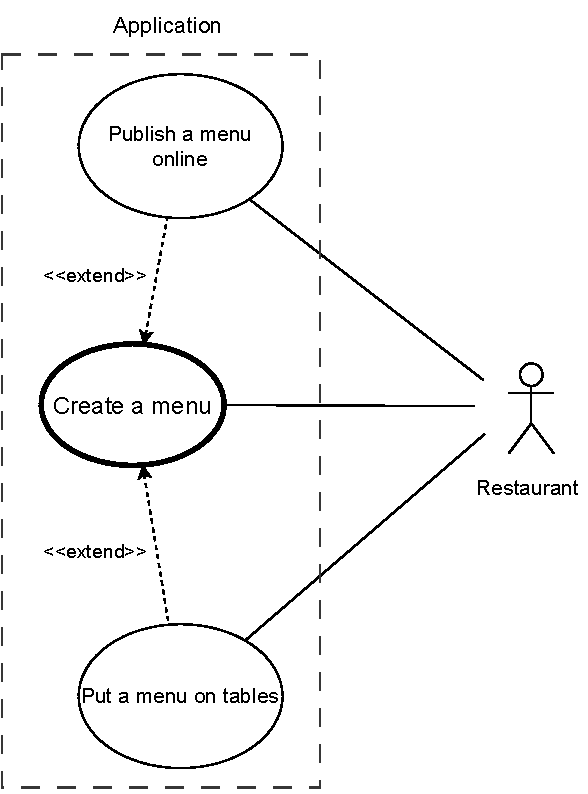
\includegraphics[width=0.62\linewidth]{master-thesis/img/use-cases/use_cases_restaurant_publish_menu}
  \caption{Restaurant offer use cases}
\end{figure}

\begin{figure}[h]
  \centering
  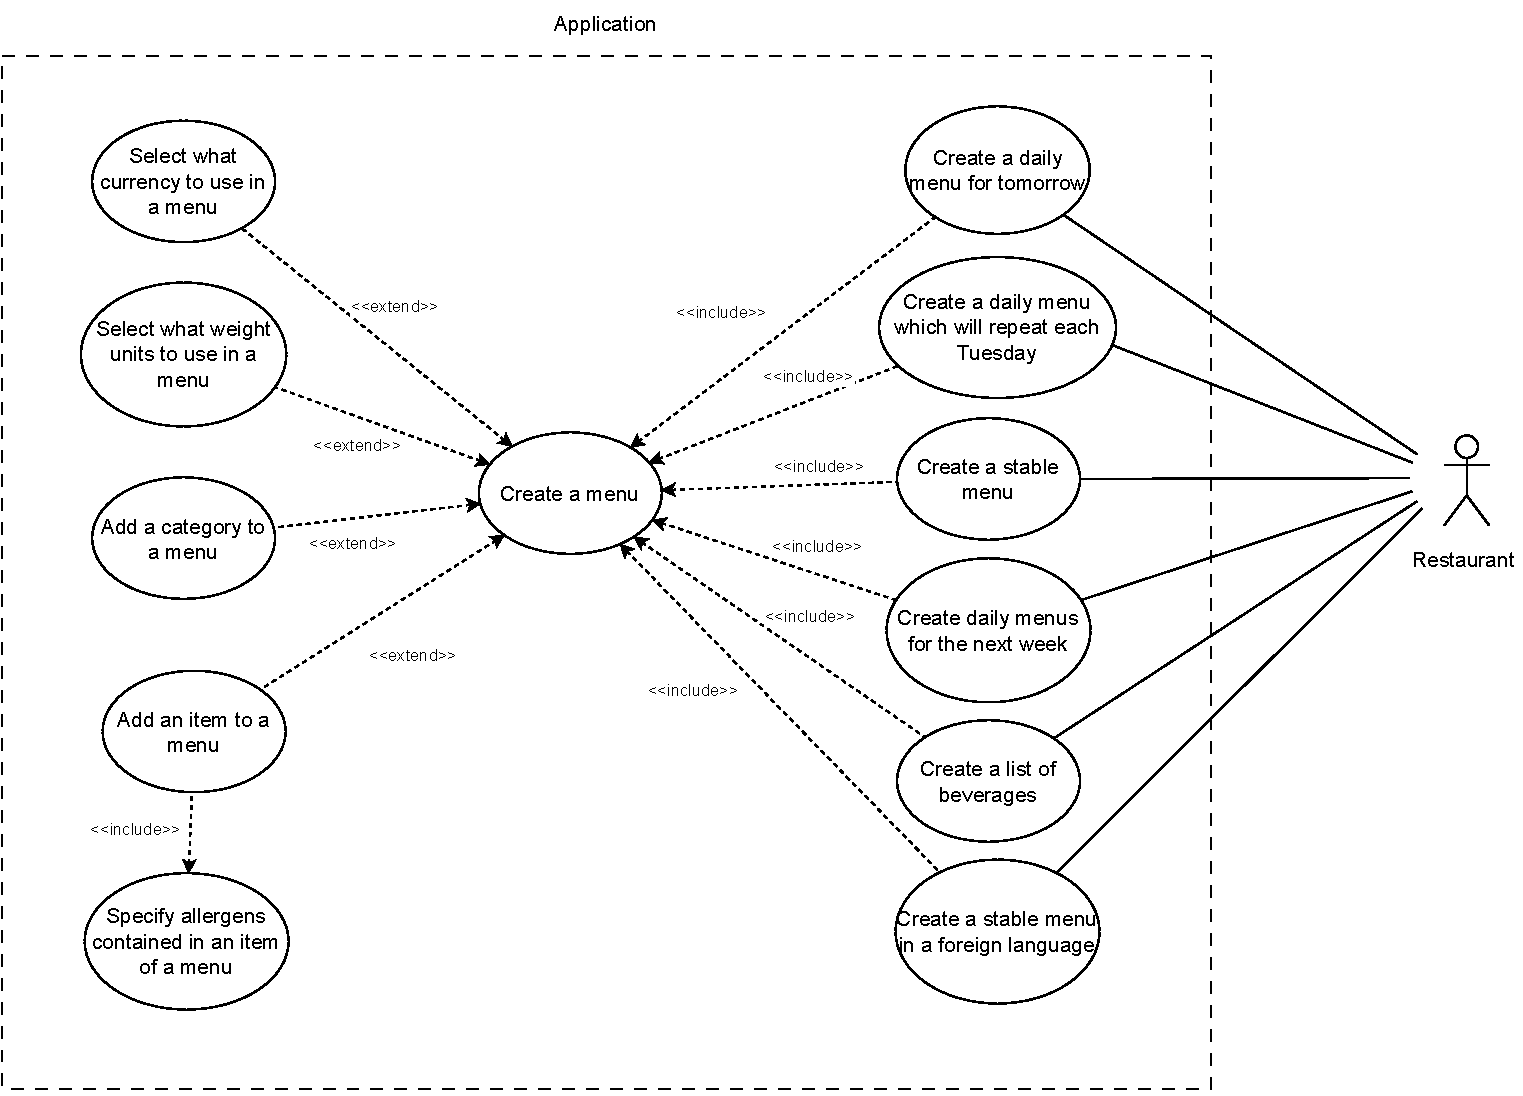
\includegraphics[width=0.62\linewidth]{master-thesis/img/use-cases/use_cases_restaurant_create_menu}
  \caption{Restaurant menu creation use cases}
\end{figure}

\begin{figure}[h]
  \centering
  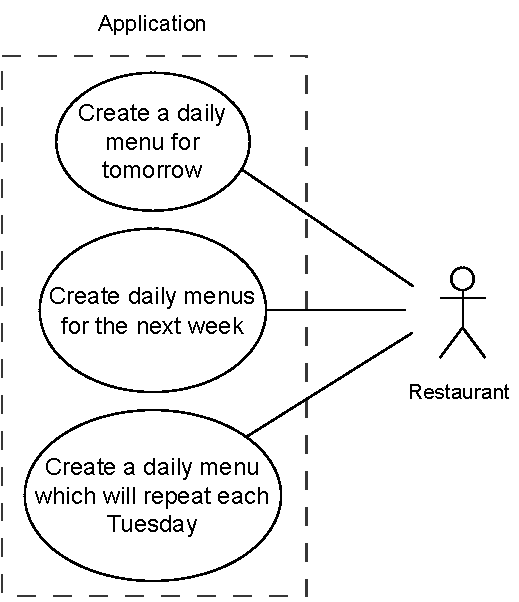
\includegraphics[width=0.62\linewidth]{master-thesis/img/use-cases/use_cases_restaurant_create_daily_menu}
  \caption{Restaurant daily menu creation use cases}
\end{figure}
